\section{Chapter Review}

\begin{puzzle}
    Is the matrix given below a transition matrix for a Markov chain? Explain.
    \begin{enumerate}
        \item $\begin{bmatrix} .1 & .4 & .5 \\ .5 & -.3 & .8 \\ .3 & .4 & .3 \end{bmatrix}$
        \item $\begin{bmatrix} .2 & .6 & .2 \\ 0 & 0 & 0 \\ .3 & .4 & .5 \end{bmatrix}$
    \end{enumerate}
\end{puzzle}

\begin{puzzle}
    A survey of computer buyers indicates that if a person buys an Apple computer, there is an 80\% chance that their next purchase will be an Apple, while owners of an IBM will buy an IBM again with a probability of .70. The buying habits of these consumers are represented in the transition matrix below.

    \[
        \begin{tabular}{lc|cc}
                 &       & To    &     \\
                 &       & Apple & IBM \\
            \hline
            From & Apple & .80   & .20 \\
                 & IBM   & .30   & .70 \\
        \end{tabular}
    \]

    Find the following probabilities:
    \begin{enumerate}
        \item The probability that a present owner of an Apple will buy an IBM as his next computer.
        \item The probability that a present owner of an Apple will buy an IBM as his third computer.
        \item The probability that a present owner of an IBM will buy an IBM as his fourth computer.
    \end{enumerate}
\end{puzzle}



\begin{puzzle}
    Professor Trayer either teaches Finite Math or Statistics each quarter. She never teaches Finite Math two consecutive quarters, but if she teaches Statistics one quarter, then the next quarter she will teach Statistics with a $1/3$ probability.

    \begin{enumerate}
        \item Write a transition matrix for this problem.
        \item If Professor Trayer teaches Finite Math in the Fall quarter, what is the probability that she
              will teach Statistics in the Winter quarter.
        \item If Professor Trayer teaches Finite Math in the Fall quarter, what is the probability that she
              will teach Statistics in the Spring quarter.
    \end{enumerate}
\end{puzzle}

\begin{puzzle}
    The transition table for switching academic majors each quarter by students at a university is given below, where Science, Business, and Liberal Arts majors are denoted by the letters S, B, and A, respectively.

    \[
        \begin{tabular}{lc|ccc}
                 &   &    & To &    \\
                 &   & S  & B  & A  \\
            \hline
                 & S & .6 & .3 & .1 \\
            From & B & .1 & .7 & .2 \\
                 & A & .1 & .1 & .8 \\
        \end{tabular}
    \]

    \begin{enumerate}
        \item Find the probability of a science major switching to a business major during their first quarter.
        \item Find the probability of a business major switching to a Liberal Arts major during their second
              quarter.
        \item  Find the probability of a science major switching to a Liberal Arts major during their third
              quarter.
    \end{enumerate}

\end{puzzle}

\begin{puzzle}
    Determine whether the following matrices are regular Markov chains.

    \begin{enumerate}
        \item \[
                  \begin{bmatrix}
                      1  & 0  \\
                      .3 & .7
                  \end{bmatrix}
              \]
        \item \[
                  \begin{bmatrix}
                      .2 & .4 & .4 \\
                      .6 & .4 & 0  \\
                      .3 & .2 & .5
                  \end{bmatrix}
              \]
    \end{enumerate}
\end{puzzle}

\begin{puzzle}
    John Elway, the football quarterback for the Denver Broncos, calls his own plays. At every play he has to decide to either pass the ball or hand it off. The transition table for his plays is given below, where \(P\) represents a pass and \(H\) a handoff.

    \[
        \begin{tabular}{c|cc}
              & P  & H  \\
            \hline
            P & .6 & .4 \\
            H & .8 & .2 \\
        \end{tabular}
    \]

    \begin{enumerate}
        \item If John Elway threw a pass on the first play, what is the probability that he will handoff on the third play?
        \item Determine the long term play distribution.
    \end{enumerate}
\end{puzzle}


\begin{puzzle}
    Company I, Company II, and Company III compete against each other, and the transition table for people switching from company to company each year is given below.

    \[
        \begin{tabular}{c|ccc}
                       & \text{I} & \text{II} & \text{III} \\
            \hline
            \text{I}   & .6       & .2        & .2         \\
            \text{II}  & .3       & .5        & .2         \\
            \text{III} & .3       & .3        & .4         \\
        \end{tabular}
    \]

    \begin{enumerate}
        \item If the initial market share is 20\% for Company I, 30\% for Company II, and 50\% for Company III, what will the market share be after the next year?
        \item If this trend continues, what is the long range expectation for the market?
    \end{enumerate}
\end{puzzle}


\begin{puzzle}
    Given the following absorbing Markov chain.

    \[
        T = \begin{bmatrix}
            1  & 0  & 0  & 0  \\
            0  & 1  & 0  & 0  \\
            .2 & .3 & .4 & .1 \\
            .4 & .1 & .1 & .4 \\
        \end{bmatrix}
    \]

    \begin{enumerate}
        \item Identify the absorbing states.
        \item Write the solution matrix.
        \item Starting from state 4, what is the probability of eventual absorption in state 1?
        \item Starting from state 3, what is the probability of eventual absorption in state 2?
    \end{enumerate}
\end{puzzle}




\begin{puzzle}\label{puzzle_rat_maze_again}
    A rat is placed in the maze shown below, and it moves from room to room randomly. From any room, the rat will choose a door to the next room with equal probabilities. Once it reaches room 1, it finds food and never leaves that room. And when it reaches room 6, it is trapped and cannot leave that room. What is the probability that the rat will end up in room 1 if it was initially placed in room 3?

    % TODO Better version of this
    \begin{center}
        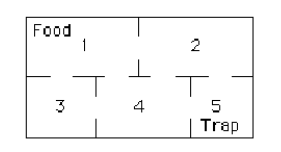
\includegraphics{chapters/markov_hw/section03/maze.png}
    \end{center}
\end{puzzle}

\begin{puzzle}
    In Puzzle \ref{puzzle_rat_maze_again}, what is the probability that the rat will end up in room 6 if it was initially in room 2?
\end{puzzle}